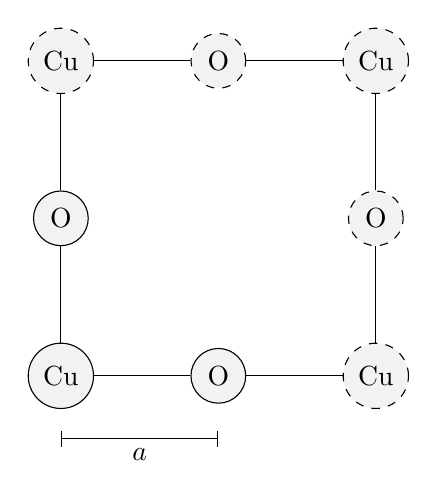
\begin{tikzpicture}[
        atom/.style={
            circle,
            fill=black!5,
            draw=black,
        },
        ghost/.style={
            circle,
            fill=black!5,
            draw=black,
            dashed,
        },
        scale=2,
    ]

    \node[atom]  (a1) at (0, 0) {Cu};
    \node[atom]  (a2) at (1, 0) {O};
    \node[ghost] (a3) at (2, 0) {Cu};
    \node[ghost] (a4) at (2, 1) {O};
    \node[ghost] (a5) at (2, 2) {Cu};
    \node[ghost] (a6) at (1, 2) {O};
    \node[ghost] (a7) at (0, 2) {Cu};
    \node[atom]  (a8) at (0, 1) {O};

    \draw (a1) -- (a2) -- (a3) -- (a4) -- (a5) -- (a6) -- (a7) -- (a8) -- (a1);

    \draw[|-|] (0, -.4) -- node[midway, below] {$a$} ++(1, 0);

\end{tikzpicture}
